\documentclass{article}

\usepackage{tikz}
\usetikzlibrary{decorations.pathreplacing}
\usepackage{ tipa }
\usepackage{amsmath}
\usepackage{amssymb}
\usepackage{upgreek}
\usepackage{graphicx}
\usepackage[font={footnotesize,it}]{caption}
\usepackage[margin=0.5in]{geometry} %remove comment after todonotes are dealt with
\usepackage[textwidth=1.5in]{todonotes}
\usepackage{parskip}

\usepackage{mathtools}
\DeclarePairedDelimiter\abs{\lvert}{\rvert}%

\begin{document}
\title{Water Contact Simplification}
\author{Mahdi Khoramshahi}
\maketitle




Based on literature, force on generated foot pad can be calculated as follow:
\begin{align}\label{eq:spliting}
	F_w &= C_{D}^* \rho \int_{-R}^{-R+2sR} \sqrt{( R^2-z^2)} (2gh(z)+v(z)\abs{v(z)})dz\\
	h(z)&= (y_{water}-y_{BF})(1-\frac{z+R}{2sR})\\
	v(z) &= \vec{V}(z)^{'} \cdot \vec{n}\\
	s   &= \frac{y_{water}-y_{BF}}{y_{TF}-y_{BF}}
\end{align}

Equation could be more simple if  position of center of foot ($y_c$),foot angle ($\theta$), normal linear and angular velocity at center of foot($v_n$,$\dot{\theta}$). Therefore, change of variables is: 

\begin{align}\label{eq:spliting}
	\left( y_{TF},y_{BF} \right) &\Leftrightarrow \left( y_c, \theta \right)\\
	y_{TF} &= y_c + R~\mathrm{sin}(\theta)\\
	y_{BF} &= y_c - R~\mathrm{sin}(\theta)
\end{align}

now we can rewrite 



\begin{align}\label{eq:spliting}
	h(z)&= (y_{water}-y_{c})-z\mathrm{sin}\theta\\
	v(z) &= v_n + \dot{\theta}z\\
	s   &= 0.5+\frac{y_{water}-y_c}{2R\mathrm{sin}\theta}
\end{align}

Upper boundary for integral can be simplified this way:

\begin{align}\label{eq:spliting}
	r_u &= -R+2sR \\
	r_u &= -R+ 2 \left( 0.5+\frac{y_{water}-y_c}{2R\sin\theta} \right) R \\
	r_u &= \frac{ \left( y_{water}-{y_c} \right) }{\mathrm{sin}\theta}
\end{align}

Integral can be seen as two less complicated integral:
\begin{align}\label{eq:spliting}
	F_w =& C_{D}^* \rho \int_{-R}^{-R+2sR} \sqrt{( R^2-z^2)} (2gh(z)+v(z)\abs{v(z)})dz\\
		=& ~C_{D}^* \rho \int_{-R}^{-R+2sR} \sqrt{( R^2-z^2)} (2gh(z))dz \\
		 & + C_{D}^* \rho \int_{-R}^{-R+2sR} \sqrt{( R^2-z^2)} (v(z)\abs{v(z)})dz
\end{align}

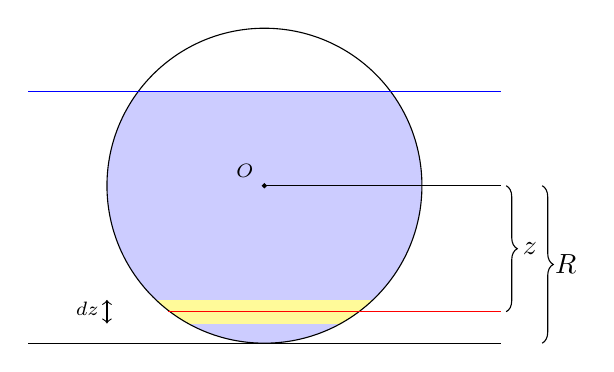
\begin{tikzpicture}

  %color one strip
  \begin{scope}
    \clip (0,0) circle (2cm);
    \fill[blue!20] (2cm,1.2cm) rectangle (-2cm, -2cm);
    \fill[yellow!40] (2cm,-1.45cm) rectangle (-2cm, -1.75cm);
  \end{scope}

  %outer line
  \draw (0,0) circle (2cm);

	% water level
	\draw (-3,1.2) -- (3,1.2) [blue]; 
	% to z
	\draw (-1.22,-1.6) -- (3,-1.6) [red]; 
	% to end
	\draw (-3,-2) -- (3,-2) [black]; 
	% to center
	\draw (0,0) -- (3,0) [black];
	\node (0,0)[draw=none,fill=none] [label={[xshift=-.25cm, yshift=-0.15cm] {\scriptsize $O$}}] {};
    \draw (0,0) circle (0.025cm) [fill= black];

	\draw [<->] (-2,-1.45) -- (-2,-1.75)   node [draw=none,fill=none] [label={[xshift=-.25cm, yshift=-0.15cm] {\scriptsize $dz$}}] {};

	\draw [decorate,decoration={brace,amplitude=4pt,mirror},xshift=2pt,yshift=0pt](3,-1.6) -- (3,0) node [black,midway,xshift=.3cm] {$z$};
	\draw [decorate,decoration={brace,amplitude=4pt,mirror},xshift=15pt,yshift=0pt](3,-2) -- (3,0) node [black,midway,xshift=.3cm] {$R$};

\end{tikzpicture}


We are going to use analytic solution to following integrals. 
\begin{align}\label{eq:two_int}
I_k(r) &=\int _{-R}^{r} ( {\it a} z+{\it b} )~ \sqrt{R^2-z^2}dz\\
I_b(r) &=\int _{-R}^{r} ( {\it a} z+{\it b} )^2 \sqrt{R^2-z^2}dz
\end{align}

for sake of simplicity we define following function for $-R<r<R$.
\begin{align}\label{eq:simplie}
l(r) &= \sqrt{R^2-r^2}\\
\phi(r) &= \arcsin(\frac{r}{R})
\end{align}

The analytic solution to integral in \eqref{eq:two_int} is as follow:
\begin{align}\label{eq:integrals}
	  \int _{-R}^{r} (az+b ) l(z)dz &=  \frac{\pi b R^2}{4} - \frac{a{l(r)}^3}{3}  +\frac{b R^2\phi(r)}{2}+ \frac{brl(r)}{2}\\
	                                &=  \frac{bR^2}{2} \left(\phi(r) + \frac{\pi}{2}\right) + \frac{br}{2} l(r) - \frac{a}{3} l(r)^3 \\
	  \int _{-R}^{r} (az+b)^2 l(z)dz &=  \frac{\pi R^2}{16}(a^2 R^2 + 4 b^2) + \frac{R^2 \phi(r)}{8}(a^2 R^2 + 4b^2) + \frac{rl(r)}{8} (a^2 R^2 + 4b^2)-
	  al(r)^3 (\frac{ar}{4}+\frac{2b}{3})\\
	  &=  \frac{1}{8}(a^2 R^2 + 4 b^2) \left(\left(\phi(r)+\frac{\pi}{2}\right)R^2 + rl(r)\right) - al(r)^3 (\frac{ar}{4}+\frac{2b}{3}) 
\end{align}

Now we are going to deal with absolute in following integral
\begin{align}\label{eq:two_int}
\tilde{I}_b = \int _{-R}^{r} v(z) \abs{v(z) }~l(z)dz
\end{align}
luckily $v(z)$ only change once over $z$; let assume that it happens at $r_0$. we first define: 

\begin{align}\label{eq:two_int}\
	v(r_0) &= 0\\	
	v_n + \dot{\theta}r_0 &= 0\\
	&\Rightarrow r_0 = ~ \frac{v_n}{\dot{\theta}}~, ~(~\dot{\theta} \neq 0)
\end{align}

\begin{align}\label{eq:two_int}\
	S(z)  &= \mathrm{sign}\left(v(z)\right)\\
	r_0^+ &= r_o + \epsilon\\
	r_0^- &= r_o - \epsilon
\end{align}

we can rewrite the integral as:
\begin{align}\label{eq:two_int}
\tilde{I}_b &= S(r_0^-) \int _{-R}^{r_0} v(z)^2~ l(z)dz + S(r_0^+) \int _{r_0}^{r} v(z)^2~ l(z)dz \\
			&= S(r_0^-) \int _{-R}^{r_0} v(z)^2~ l(z)dz + S(r_0^+) \left( \int _{-R}^{r} v(z)^2~ l(z)dz ) -  
			\int _{-R}^{r_0} v(z)^2~ l(z)dz \right)\\
			&= \left( (S(r_0^-)-S(r_0^+) \right)  \int _{-R}^{r_0} v(z)^2~ l(z)dz + S(r_0^+) \int _{-R}^{r} v(z)^2~ l(z)dz ) \\
			&= \left( (S(r_0^-)-S(r_0^+) \right)  I_b(r_0) + S(r_0^+) I_b(r)
\end{align}


\end{document}
